\chapter{Sintassi}

\section{Prologo}

La sintassi è il fenomeno che permette di percepire come corrette certe frasi e come scorrette altre. I linguisti separano la sintassi in:
\begin{itemize}
  \item Competence. 
  \item Performance.
\end{itemize}

\dfn{Competence}{
  La competence rappresenta la grammatica formale. Una conoscenza pura linguistica.
}

\nt{La linguistica dovrebbe occuparsi della competence.}

\dfn{Performance}{
La performance rappresenta un algoritmo di parsing. Come si utilizza la conoscenza pura.
}

\nt{È importante conoscere la grammatica formale per poterla utilizzare con un algoritmo.}

\subsection{Grammatiche Generative}

\dfn{Sistemi di Riscrittura}{
  Sistema formale della tradizione matematica utilizzato come base da Chomsky.
}

\begin{figure}[h]
    \centering
    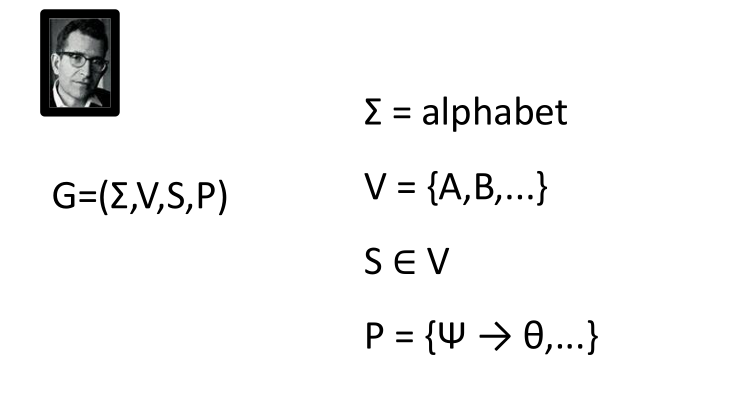
\includegraphics[scale=0.6]{03/gen.png}
    \caption{Grammatiche Generative.}
\end{figure}

\begin{itemize}
  \item Le grammatiche generative modellano il linguaggio naturale come un linguaggio formale. 
  \item L'albero di derivazione può modellare la struttura sintattica della frase. 
\end{itemize}

\paragraph{Le grammatiche context free:}

\begin{itemize}
  \item Costituenza: i costituenti rappresentano i simboli non terminali V. 
  \item Relazione grammaticale. 
  \item Sottocategorigazioni.
\end{itemize}

\nt{Chomsky dimostrò che le lingue naturali sono \fancyglitter{almeno} context free.}

\begin{figure}[h]
    \centering
    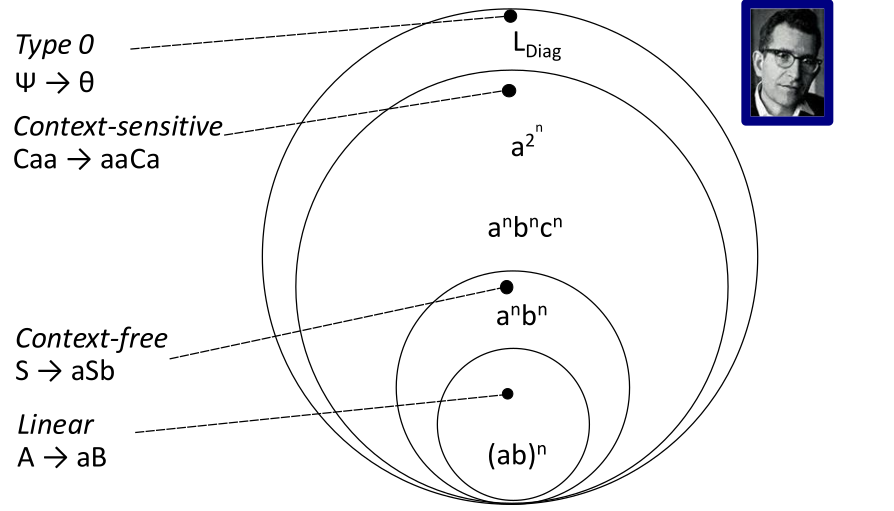
\includegraphics[scale=0.4]{03/chomsky.png}
    \caption{Gerarchia di Chomsky.}
\end{figure}

\nt{Questa gerarchia mette in "ordine" le complessità di vari tipi di linguaggi.
  Le lingue naturali si trovano nel \fancyglitter{context-sensitive}, o meglio, nelle \fancyglitter{mildly-context-sensitive} ($a^n*b^n*c^n$). 
}

\subsection{Mildly-context-sensitive}

\dfn{Proprietà di Crescita Costante}{
  Un languaggio $L$ cresce costantemente se c'è una costante $c_0$ e un insieme finito di costanti $C$ tale che per ogni $w \epsilon L$ dove $|w| > c_0$ tale che $|w| = |w'| + c$ per qualche $c \epsilon C$. 
}

\nt{Questa proprietà è la versione formale dell'intuizione linguistica che una frase appartenente a un linguaggio naturale può essere costruita da un insieme finito di strutture usando la stessa operazione lineare.}

\section{La Performance e i costituenti}

\subsection{Approcci al Parsing}

\paragraph{Parser anatomy (Steedman):}

\begin{itemize}
  \item Competence: Context-free, TAG, CCG, Dipendenza, etc.
  \item Algoritmo: 
    \begin{itemize}
      \item Strategia di ricerca: top-down, bottom-up, left-to-right, etc. 
      \item Organizzazione della memoria: back-tracking (approccio in profondità, PROLOG), programmazione dinamica (approccio in ampiezza).
    \end{itemize}
  \item Oracolo: probabilistico, a regole, etc.
\end{itemize}

\nt{L'oracolo serve per via dell'ambiguità delle lingue naturali. Decide quale regola applicare prima secondo suoi criteri.}

\paragraph
{Fonti di informazioni:}

\begin{itemize}
  \item Grammatica $\rightarrow$ parsing diretto dai goal $\rightarrow$ top-down. 
    \begin{itemize}
      \item Solo ricerche che possono portare a risposte corrette, cioè con
radice S. 
      \item Comporta la creazione di alberi non compatibili con le parole. 
      \item Razionalisti.
    \end{itemize}
  \item Frase $\rightarrow$ parsing diretto dai dati $\rightarrow$ bottom-up. 
    \begin{itemize}
      \item Solo ricerche compatibili con le parole. 
      \item Comporta la creazione di alberi non corretti. 
      \item Empiristi.
    \end{itemize}
\end{itemize}







